%%%%%%%%%%%%%%%%%%%%%%%%%%%%%%%%%%%%%%%%%%%
%
% szablon pracy licencjackiej 
% korzystający ze stylu pracalicmgr.cls
% 2017.03.22 K. Turzynski
% 2017.03.01 P. Durka durka@fuw.edu.pl 
% na podstawie pliku J. Żygierewicz 2016
%
%%%%%%%%%%%%%%%%%%%%%%%%%%%%%%%%%%%%%%%%%%%



\documentclass{pracalicmgr}
\usepackage{polski}
\usepackage[utf8]{inputenc}
\usepackage{float}
\usepackage{booktabs}
\usepackage{hyperref}
\usepackage{url}
\usepackage{caption}
\usepackage{subcaption}
\usepackage{graphicx}
\usepackage[backend=bibtex]{biblatex}

\sloppy
\frenchspacing
\addbibresource{bibliografia.bib}

\author{Agnieszka Ciepielewska}

\nralbumu{385537}

\title{Zastosowanie uczenia maszynowego do identyfikacji leptonów tau w eksperymencie CMS}

\tytulang{Application of machine learning for tau leptons identification in the CMS experiment}

\kierunek{Fizyka w ramach Międzywydziałowych Indywidualnych
Studiów Matematyczno-Przyrodniczych}

% \specjalnosc{}

\opiekun{dr hab. Artur Kalinowski \\ Zakład Cząstek i Oddziaływań Fundamentalnych \\ Instytut Fizyki Doświadczalnej}

%\dziedzina{13.200}
\dziedzina{13.2 Fizyka}

\date{$<$TODO: miesiąc-i-rok-złożenia-pracy$>$}

\keywords{$<$TODO: wykaz maksymalnie 10 słów swobodnie wybranych$>$}



\begin{document}


    \maketitle
    \let\cleardoublepage\clearpage
    
    \begin{abstract}
    %TODO
$<$Krótkie (maks. 800 znaków) streszczenie pracy, na przykład:

Lorem ipsum – tekst składający się z łacińskich i quasi-łacińskich wyrazów, mający korzenie w klasycznej łacinie, wzorowany na fragmencie traktatu Cycerona „O granicach dobra i zła” (De finibus bonorum et malorum) napisanego w 45 r. p.n.e. Tekst jest stosowany do demonstracji krojów pisma (czcionek, fontów), kompozycji kolumny itp. Po raz pierwszy został użyty przez nieznanego drukarza w XVI w.

Tekst w obcym języku pozwala skoncentrować uwagę na wizualnych aspektach tekstu, a nie jego znaczeniu.

Cytat z {\tt https://pl.wikipedia.org/wiki/Lorem\_ipsum}
$>$

    \end{abstract}

    \tableofcontents
    
    \chapter*{Cel pracy}
    \addcontentsline{toc}{chapter}{Cel pracy}
    %TODO
    \chapter{Wstęp}
    \label{ch:wstep}
	%TODO    
    Tutaj piszemy informacje wprowadzające w tematykę  pracy, potrzebne do zrozumienia treści.       
    \section{Leptony tau}
    
    Leptony tau	odgrywają istotną rolę w wielu eksperymentach fizycznych. Jednym z ważniejszych jest badanie bozonu Higgsa w rozpadzie $H \rightarrow \tau\tau$. Jednak z powodu krótkiego czasu życia $\tau = 2.9 \cdot 10^{-13}~\mathrm{s}$ \cite{particle_physics}, one również nie są wykrywane bezpośrednio w eksperymentach, ale obserwuje się ich produkty rozpadu. Taony są najcięższymi z leptonów i przy swojej masie $m_\tau = 1.776 ~\mathrm{GeV/c}^2$ \cite{particle_physics} jako jedyne są w stanie rozpadać się hadronowo. Z tabeli \ref{tab:kanaly_rozpadu} widać, że dzieje się tak w około $2/3$ przypadków. Sprawia to problemy przy ich identyfikacji, ponieważ łatwo jest je pomylić z jetami hadronowymi (ang. \textit{QCD jets}).
    
	\begin{table}[H]
	\centering
	\caption{Główne kanały rozpadu taonów wraz z prawdopodobieństwem \cite{tauid13, particle_physics}. Tutaj $h$ oznacza zarówno mezony $\pi$ jak i $K$.}
	\label{tab:kanaly_rozpadu}
	\begin{tabular}{lr}
	\toprule
	Rozpad & Prawdopodobieństwo [\%] \\
	\midrule
	\multicolumn{2}{c}{Rozpady leptonowe} \\
	\midrule
	$\tau^- \rightarrow e^-\bar{\nu}_{e}\nu_{\tau}$ & $17.8$ \\
	$\tau^- \rightarrow \mu^-\bar{\nu}_{\mu}\nu_{\tau}$ & $17.4$ \\
	\midrule
	\multicolumn{2}{c}{Rozpady hadronowe} \\
	\midrule
	$\tau^- \rightarrow h^- \pi^0 \nu_{\tau}$ & $25.9$ \\
	$\tau^- \rightarrow h^-\nu_{\tau}$ & $11.5$ \\
	$\tau^- \rightarrow h^- h^+ h^- \nu_{\tau}$ & $9.8$ \\
	$\tau^- \rightarrow h^- \pi^0 \pi^0 \nu_{\tau}$ & $9.5$ \\
	$\tau^- \rightarrow h^- h^+ h^- \pi^0 \nu_{\tau}$ & $4.8$ \\
	Inne & $3.3$ \\	
	\bottomrule
	\end{tabular}
	\end{table}
        
    \section{Detektor CMS}
	Detektor CMS (\textit{Compact Muon Solenoid}) znajduje się w Wielkim Zderzaczu Hadronów (LHC) w CERN-ie. Jego główne elementy to: nadprzewodząca cewka wytwarzająca pole magnetyczne o indukcji 3.8 T, detektory krzemowe, kalorymetr elektromagnetyczny (ECAL), kalorymetr hadronowy (HCAL) i komora jonizacyjna do wykrywania mionów. 
	
	Detektor krzemowy, pokrywający przedział pseudopospieszności $|\eta| < 2.5$, składa się z dwóch rodzajów detektorów: pikselowych i paskowych. Korpus centralny składa się z trzech warstw detektorów pikselowych oraz jedenastu warstw detektorów paskowych, natomiast końcówki z jedenastu dysków, z czego dwa zawierają detektory pikselowe, a pozostałe detektory paskowe \cite{cms_technical}. Tor lotu hadronów jest rekonstruowany ze skutecznością 80-90\% w zależności od pędu poprzecznego i pseudopospieszności $\eta$. Detektory krzemowe mają grubość od 0.4 do 2.0 długości drogi radiacyjnej ($X_0$), także fotony z dużym prawdopodobieństwem konwertują wewnątrz detektora na pary $e^+e^-$ \cite{tauid13}.
	
	Kalorymetr ECAL jest zrobiony ze scyntylacyjnych kryształów stolzytu (PbWO$_4$). Posiada ponad 61000 kryształów w korpusie centralnym, pokrywającym $|\eta| < 1.48$ oraz ponad 7300 kryształów na końcach detektora, pokrywających $|\eta| < 3.0$. Stolzyt posiada krótką drogę radiacyjną ($X_0 = 0.89$ cm), krótki promień Molièra (2.2 cm) oraz szybko wyświeca światło (80\% światła jest wyświecane w 25 ns). Dzięki temu dobrze rozdziela kaskady, więc jest często wykorzystywany do budowy kalorymetrów \cite{cms_technical}.
	
	Na zewnątrz ECAL znajduje się kalorymetr hadronowy HCAL zawierający mosiądz i plastik. Mosiądz został wybrany ze względu na krótką drogę swobodną (\textit{interaction length}) hadronów oraz słabe właściwości magnetyczne.
Tak samo jak ECAL pokrywa obszar $|\eta| < 3.0$. Jego grubość to od siedmiu do jedenastu dróg swobodnych w zależności od $\eta$. Natomiast dla $3.0 < \eta < 5.0$ używany jest stalowo kwarcowy kalorymetr przedni (ang. \textit{Hadron Forward}) \cite{cms_technical}.
	
	Detektor mionowy składa się z trzech rodzajów komór gazowych. W części centralnej ($|\eta| < 1.2$) używane są komory \textit{drift tube} (DT), w części końcowej ($|\eta| < 2.4$), pole magnetyczne nadal jest duże, ale niejednolite, używa się \textit{cathode strip chambers} (CSC). Dodatkowo we wszystkich miejscach są zastosowane \textit{resistive plate chambers} (RPC). RPC zapewnia dobrą dokładność czasową, natomiast DT i CSC dobrą dokładność pozycyjną \cite{cms_technical}.
	
	\section{Sieci neuronowe}
	Sieci neuronowe to klasa modeli uczenia maszynowego stosowana w uczeniu nadzorowanym \cite{dl}. Na podstawie danych treningowych zawierający zmienne objaśniające i objaśniane model uczy się zależności występujących między tymi zmiennymi. Dzieki temu możliwe jest stosowanie modelu do predykcji zmiennych objaśnianych na podstawie nowych obserwacji.
	
	Sieci neuronowe składają się z warstw. Podstawową warstwą używaną w sieciach neuronowych jest warstwa gęsta (\textit{dense layer} lub \textit{fully connected layer}). Warstwa gęsta przyjmuje na wejściu wektor, a na wyjściu zwraca wektor ustalonej wielkości, niekoniecznie tego samego rozmiaru. Jest to warstwa bardzo generyczna, jednak jej minusem jest duża liczba parametrów (sieć długo się trenuje, zajmuje dużo miejsca i może gorzej generalizować \cite{dl}). Każda warstwa gęsta składa się z dwóch podstawowych elementów: transformacji liniowej oraz funkcji nieliniowej, zwanej funkcją aktywacji. Każda regresja liniowa posiada wagi $w_i$ oraz przesunięcia $b_i$ (\textit{bias}). Wyjście z warstwy definiowane jest jako: $$y = f(x^TW + b),$$ gdzie $x$ to wektor wejściowy, $f$ - funkcja aktywacji, nie zmieniająca wymiaru wektora, $W$ - macierz wag warstwy, $b$ - wektor przesunięcia. Dodanie kolejnych warstw to złożenie kolejnych takich funkcji.
	
	 Przykładowo na rysunku \ref{fig:simple} widoczne jest wejście do sieci $x$, które jest wektorem 3-elementowym. Następnie jest on transponowany i przemnażany przez macierz wag $W_1$, która jest wymiaru $3\times4$ oraz dodane jest przesunięcie $b_1$ o wymiarze $1\times4$. Na tym etapie nakłada się również funkcję aktywacji $f_1$. Kółka w warstwie ukrytej reprezentują wyjścia transformacji liniowych już po zastosowaniu funkcji aktywacji. Kolejny krok jest analogiczny, tym razem jest to jedna regresja liniowa, czyli macierz wag $W_2$ ma wymiar $4\times1$, a przesunięcie $b_2$ $1\times1$. Zatem wyjście~$y$: $$y = f_2(f_1(x^TW_1 + b_1)W_2 + b_2),$$ gdzie $f_1, f_2$ to funkcje aktywacji. Zauważmy, że nieliniowe funkcje aktywacji są konieczne, gdyż inaczej wielowarstwową sieć neuronową zawsze dałoby się sprowadzić do przypadku zwykłej transformacji liniowej odpowiednio przemnażając wagi \cite{dl}.
	
	\begin{figure}[H]
	\centering
	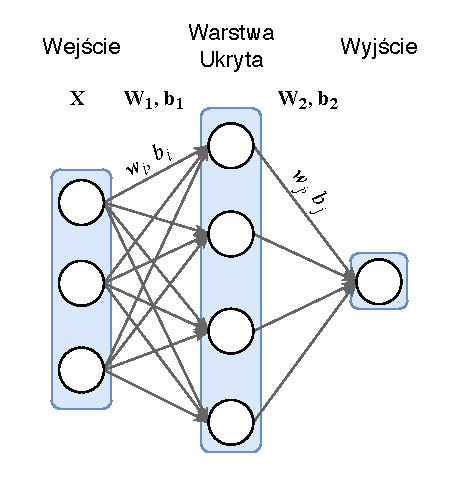
\includegraphics[width=0.5\textwidth]{simple_nn.pdf}
	\caption{Przykładowa sieć neuronowa z jedną ukrytą warstwą gęstą}
	\label{fig:simple}
	\end{figure}
	
	Następnie aby otrzymać optymalny model poszukiwane jest minimum pewnej funkcji straty $L$ (czyli miejsce, gdzie model najmniej się myli). Przez funkcję straty rozumiana jest funkcja przybliżająca błąd popełniany przez model. Minimum jest znajdowane przy pomocy gradienty funkcji $L$ względem parametrów modelu. Niestety nie da się wyznaczyć gradientu $L$ w każdym miejscu, ale można go znaleźć w punkcie, gdzie dokonywana jest predykcja. Także, aby poprawić wagi oraz przesunięcie w modelu używa się iteracyjnego algorytmu \textit{Gradient Descent}, który polega na obliczeniu gradientu funkcji straty po parametrach modelu $\nabla_{w_i}L$, a następnie aktualizowane są wagi o pewien krok w kierunku ujemnego gradientu, także dla przykładowej wagi $w$ przy $n+1$-szej iteracji (górny indeks oznacza numer iteracji): $$w^{(n+1)} \leftarrow w^{(n)} - \gamma \frac{\partial L^{(n)}}{\partial w^{(n)}},$$ gdzie $\gamma$ to tzw. stała uczenia (\textit{learning rate}) \cite{dl}. Widać, że istotne jest aby wszystkie funkcje użyte w modelu były różniczkowalne prawie wszędzie (w punktach nieciągłości pochodnej można przyjąć dowolną wartość brzegową). 
	
	W praktyce sieci neuronowe uczone są algorytmem \textit{Stochastic Gradient Descent} (SGD). Polega on na liczeniu funkcji straty dla pewnej liczby obserwacji (zwaną później \textit{batchem}), zamiast dla wszystkich obserwacji. Jednorazowe przejście przez wszystkie obserwacje nazywane jest epoką, a zazwyczaj trening modelu składa się z wielu epok.
	
	Algorytm SGD często okazuje się mało wydajny, aby otrzymać dobre rezultaty. Dlatego często stosuje się bardziej skomplikowany algorytm \textit{Adam} (\textit{Adaptive momentum}) \cite{adam}.
	
	\subsection{Funkcje aktywacji}
	Stosowane później funkcje aktywacji wraz ze wzorami:
	\begin{itemize}
	\item Sigmoid: $$S(x) = \frac{1}{1+e^{-x}},$$
	\item ReLU\cite{relu} $$ReLU(x) = \max(0, x).$$
	\end{itemize}
	
	\subsection{Warstwa \textit{batch normalization}}
	Wraz z postępem w treningu sieci wyjścia z warstw sieci mogą się zmieniać. W szczególności rozkład wyjścia może się zmieniać, do czego każda następna warstwa sieci musi się na nowo dostosowywać. Przeciwdziała temu warstwa \textit{batch normalization}, która przeskalowuje każdy batch tak aby miał tą samą średnią i odchylenie standardowe \cite{batch_norm}. Dzięki zastosowaniu \textit{batch normalization} trening sieci trwa krócej, a sieć może osiągnąć lepszą skuteczność.
	
%	\subsection{Optymalizacja \textit{Adam}}
%	Algorytm SGD często okazuje się mało wydajny, aby otrzymać dobre rezultaty. Dlatego często stosuje się algorytm \textit{Adam} (\textit{Adaptive momentum}) \cite{adam}.
	
%	Zamiast zwykłego SGD, algorytm \textit{Adam} wyznacza aktualizację wag modelu na podstawie aktualnego oraz poprzednich gradientów. Liczy statystyki $m$, $v$ oraz ostateczną zmianę wag w następujący sposób \cite{adam}:
%	$${\displaystyle m_{w}^{(n+1)}\leftarrow \beta _{1}m_{w}^{(n)}+(1-\beta _{1})\nabla _{w}L^{(n)}}$$$$
%{\displaystyle v_{w}^{(n+1)}\leftarrow \beta _{2}v_{w}^{(n)}+(1-\beta _{2})(\nabla _{w}L^{(n)})^{2}} $$$$
%{\displaystyle {\hat {m}}_{w}={\frac {m_{w}^{(n+1)}}{1-(\beta %_{1})^{t+1}}}}$$$$ {\displaystyle {\hat {v}}_{w}={\frac {v_{w}^{(n+1)}}{1-(\beta _{2})^{t+1}}}}$$$$
%{\displaystyle w^{(n+1)}\leftarrow w^{(n)}-\gamma {\frac {{\hat {m}}_{w}}{{\sqrt {{\hat {v}}_{w}}}+\epsilon }}}$$ gdzie $\beta_1, \beta_2$ to parametry, a $\epsilon$ to epsilon numeryczny.
	
	\subsection{Harmonogram stałej uczenia}
	Poza dopasowywaniem wielkości kroku aktualizacji wag zastosowanym w algorytmie \textit{Adam}, stosuje się harmonogram stałej uczenia. Polega on na zmniejszaniu stałej uczenia, gdy występuje wypłaszczenie krzywej uczenia (wartości funkcji straty w kolejnych iteracjach). Jeśli funkcja straty nie zmniejsza się przez określoną liczbę epok (przejść przez cały zbiór treningowy), stała uczenia zmniejszana jest o pewien czynnik aż osiągnie zadaną wcześniej wartość minimalną.
	
	\subsection{Miary skuteczności modeli}
	Jako, że identyfikacja taonów to problem klasyfikacji binarnej, dobrą metryką do mierzenia skuteczności modelu jest ROC AUC (\textit{Area Under Receiver Operating Characteristic Curve}) oraz sama krzywa ROC. Analizowany model przewiduje prawdopodobieństwo, czy dany rozpad zawiera taon. Aby dokonać klasyfikacji musimy ustalić próg odcięcia ponad którym zawsze zwracane jest 1 (wystąpił taon), a poniżej 0 (nie wystąpił). Wówczas można policzyć \textit{true positive rate} (TPR) oraz \textit{false positive rate} (FPR). Krzywa ROC to wykres FPR od TPR dla różnych progów odcięcie.
	
	ROC AUC to pole pod krzywą ROC. W związku z tym przyjmuje ona wartości pomiędzy 0 a 1, gdzie 0.5 to wartość osiągana przez model losowy, zaś 1 przez bezbłędny klasyfikator. ROC AUC nie jest różniczkowalna, więc nie można jej bezpośrednio wykorzystać przy treningu sieci neuronowej jako funkcji straty. Jest jednak jest przydatna przy ewaluacji oraz porównywaniu wytrenowanych modeli.
	
	Do treningu jako funkcje straty wykorzystuje się zazwyczaj binarną entropię krzyżową (\textit{binary cross entropy}) \cite{dl}, daną wzorem: $$ L(y, p) = -(y\log(p)+(1-y)\log(1-p)),$$ gdzie $y$ to prawdziwe wartości, a $p$ to predykcje modelu.
	
	\section{XGBoost}
	%TODO coś więcej (np o tym jak się dopasowuje kolejne drzewa)
	XGBoost (\textit{eXtreme Gradient Boosting}) \cite{xgboost} to implementacja algorytmu \textit{Gradient Boosting}, polegającym na budowaniu kolejnych drzew decyzyjnych (rys. \ref{fig:tree}). Każde kolejne drzewo jest tworzone aby jak najlepiej przewidywać błąd popełniany przez poprzedni zestaw drzew. Końcowa predykcja to suma wszystkich odpowiedzi drzew.
	
	\begin{figure}[h]
	\centering
	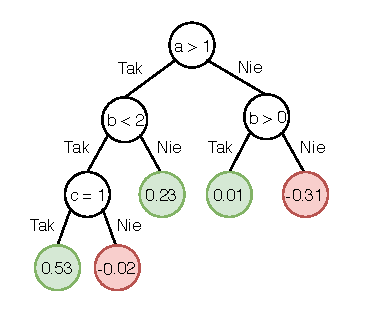
\includegraphics[width=0.5\textwidth]{tree.pdf}
	\caption{Przykładowe drzewo decyzyjne, $a, b, c$ to zmienne występujące w danych}
	\label{fig:tree}
	\end{figure}
	
    \chapter{Dane eksperymentalne oraz symulacyjne}
    \label{ch:dane}
    Dane pochodzą z symulacji zderzeń proton-proton w których został wyprodukowany bozon Higgsa i rozpadł się na parę $\tau\tau$.
Dane są wstępnie przetwarzane tak, aby pozostawić tylko najbardziej potrzebne informacje. Ostatecznie, otrzymane dane mają 19 zmiennych objaśniających \cite{cms2016reconstruction}:
	\begin{itemize}
	\item \textbf{byCombinedIsolationDeltaBetaCorrRaw3Hits} %TODO 
	\item \textbf{chargedIsoPtSum} - suma pędów naładowanych produktów rozpadu wewnątrz stożka sygnałowego.
	\item \textbf{decayDistMag} - odległość między zderzeniem $pp$ a rozpadem taonu.
	\item \textbf{decayMode} - kanał rozpadu taonu.
	\item \textbf{dxy} - odległość między zderzeniem $pp$ a rozpadem taonu w rzucie na płaszczyznę prostopadłą do osi wiązki.
	\item \textbf{dxy\_Sig} - zmienna \textbf{dxy} podzielona przez niepeność pomiaru.
	\item \textbf{eRatio} - stosunek energii taonu do energii produktów rozpadu.
	\item \textbf{flightLengthSig} - zmienna \textbf{decayDistMag} podzielona przez niepewność pomiaru. 
	\item \textbf{gjAngleDiff} - kąt między kierunkiem ruchu taonu oraz kierunkiem ruchu głównego produktu rozpadu.
	\item \textbf{hasSecondaryVertex} - informacja czy rozpad posiada wierzchołek wtórny, którym może być rozpad taonu.
	\item \textbf{ip3d} %TODO
	\item \textbf{nPhoton} - liczba protonów przypisana do rozpadu taonu.
	\item \textbf{neutralIsoPtSum} - suma pędów neutralnych produktów rozpadu wewnątrz stożka sygnałowego.
	\item \textbf{photonPtSumOutsideSignalCone} - suma pędów fotonów poza stożkiem sygnałowym.
	\item \textbf{ptWeightedDetaStrip} %TODO sprawdzić co to delta eta
	\item \textbf{ptWeightedDphiStrip} %TODO
	\item \textbf{ptWeightedDrIsolation} %TODO
	\item \textbf{ptWeightedDrSignal} %TODO
	\item \textbf{puCorrPtSum} - suma pędów cząstek neutralnych znajdujących się wewnątrz stożka sygnałowego, ale pochodząca z innych rozpadów.
	\end{itemize}
	
	Dodatkowo dane zawierają 4 zmienne będące odpowiedziami wcześniej wykorzystywanych klasyfikatorów:
	\begin{itemize}
	\item \textbf{DPFTau\_2016\_v1tauVSall} %TODO
	\item \textbf{byIsolationMVArun2v1DBnewDMwLTraw2017v2} %TODO
	\item \textbf{deepTau2017v1tauVSall} %TODO
	\item \textbf{deepTau2017v1tauVSjet} %TODO
	\end{itemize}
	
	%TODO przerobić, bo piszemy tylko o danych symulacyjnych
	Jednakże, dane eksperymentalne nie dostarczają informacji o wystąpieniu taonu. Dlatego do treningu modeli użyte zostały dane symulacyjne wytworzone metodami Monte Carlo. Symulowane są rozpady H $\rightarrow\tau\tau$, a za tło uznane są jety QCD. Dane te zawierają takie same zmienne objaśniające jak dane eksperymentalne, jednak występuje tam również zmienna objaśniana, czyli informacja binarna o wystąpieniu taonu. Przyjmuje on wartość 1 jeśli taon wystąpił (sygnał) oraz 0 jeśli nie wystąpił (tło).
	
	Na rysunku \ref{fig:diff} przedstawiono rozkład przykładowej zmiennej dla sygnału oraz tła. Widać zauważalne różnice w rozkładach, także można na podstawie tej zmiennej dokonywać klasyfikacji. Rozkłady częściowo się nakładają, więc klasyfikacja nie byłaby idealna.
	
	
	\begin{figure}[H]
	\centering
	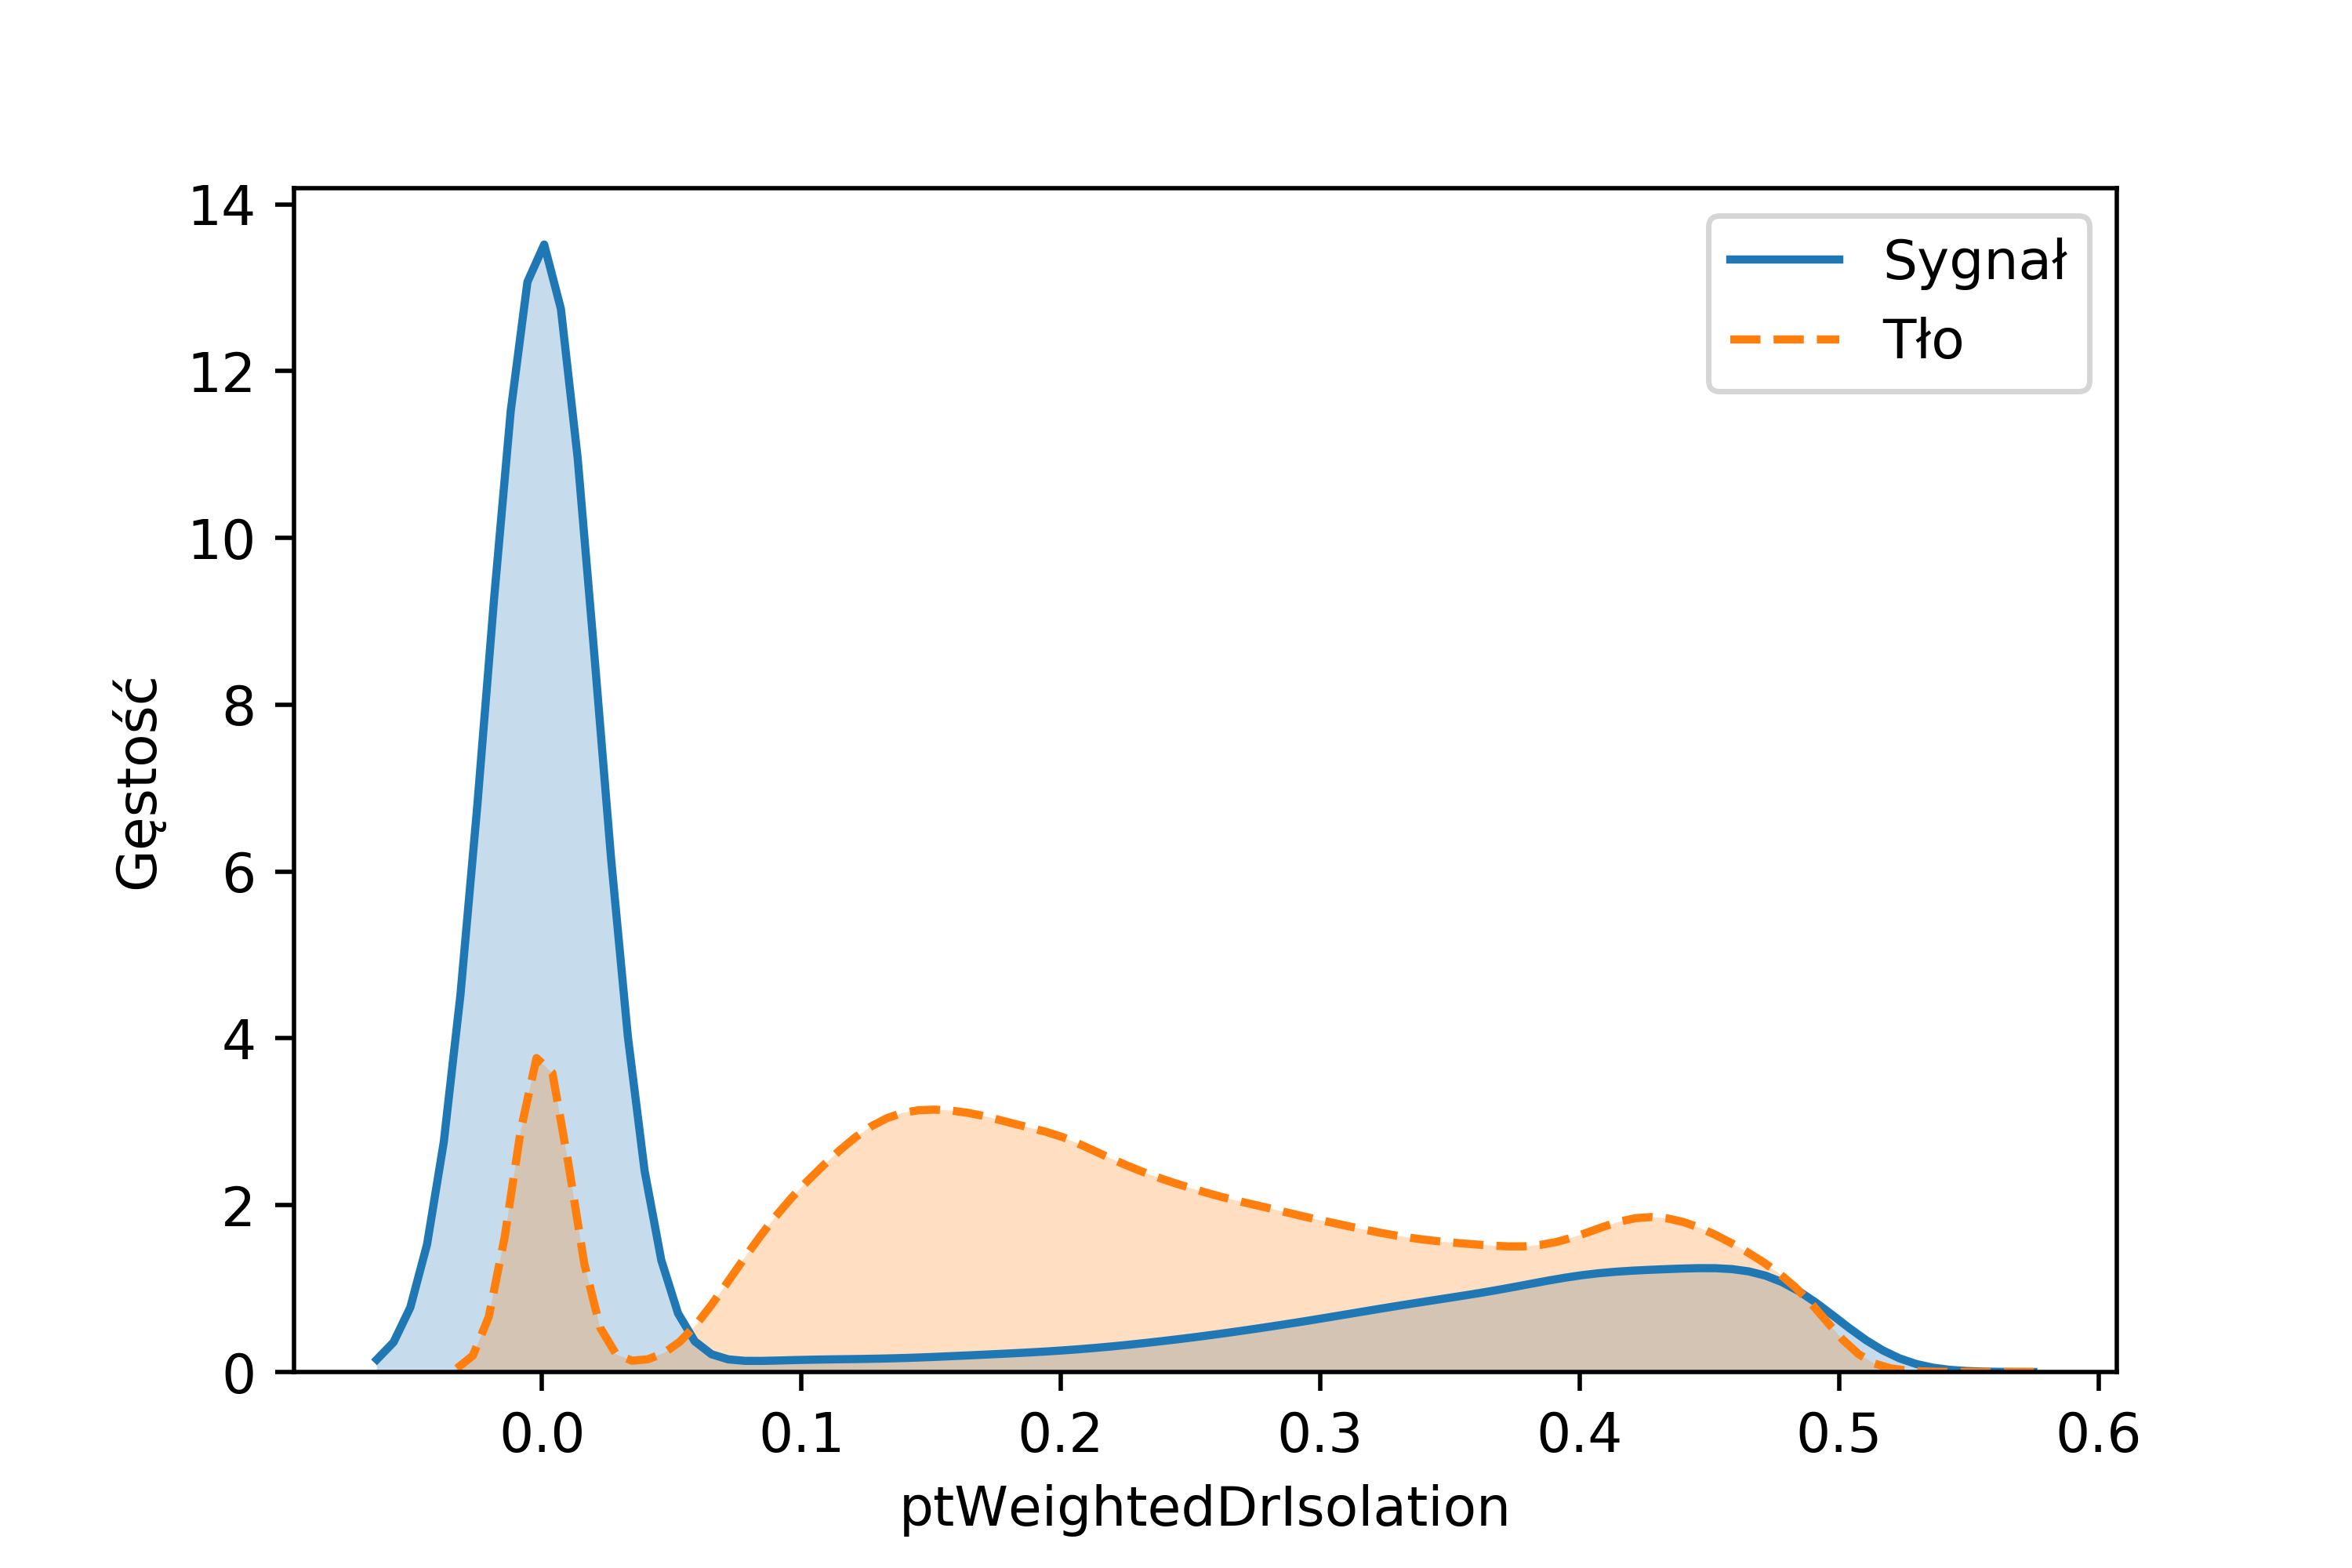
\includegraphics[width=0.75\textwidth]{difference.png}
	\caption{Różnice w rozkładzie przykładowej zmiennej dla sygnału i tła}
	\label{fig:diff}
	\end{figure}
	%TODO więcej wykresów i na czarno białe	
		
    \chapter{Architektura modeli}
	Aby dokonywać klasyfikacji sygnału zastosowano różne modele predykcyjne opierające się na metodach opisanych w rozdziale \ref{ch:wstep}.
	\section{Model oparty o same klasyfikatory}
	\label{sec:mod1}
	Prosty model, składający się z jednego neuronu, który przyjmuje jako zmienne objaśniające odpowiedzi wcześniej używanych klasyfikatorów (patrz rozdział \ref{ch:dane}). Jest to więc średnia ważona odpowiedzi klasyfikatorów, na którą nałożona jest funkcja sigmoid. Wielkość batcha została ustalona na 128, do optymalizacji został użyty algorytm \textit{Adam} ze stałą uczenia $\gamma = 10^{-3}$. Model uczony był przez cztery epoki. Później używana jest nazwa \textit{ensemble}.
	\section{Sieć neuronowa}
	\label{sec:mod2}
	Kolejny model był oparty o wszystkie zmienne objaśniające, jego architekturę przedstawiono na rysunku \ref{fig:nn1}. Składał się z sześciu warstw gęstych, o wielkości 32 neuronów każda. Jako funkcje aktywacji zastosowano funkcje ReLU. Warstwę wyjściową tworzy jeden neuron z sigmoidem jako funkcją aktywacji. Dzięki temu wyjściem sieci jest pojedyncza wartość z zakresu [0, 1]. Inne parametry zostały ustalone tak samo jak dla modelu w sekcji \ref{sec:mod1}. Ten model zwany jest później jako \textit{baseline}.
	\begin{figure}
	\centering
	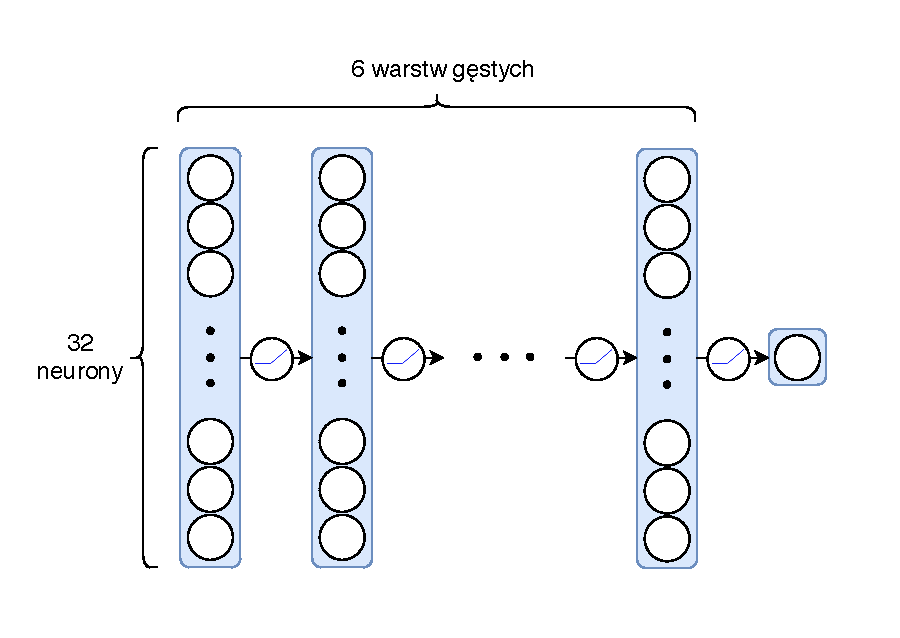
\includegraphics[width=0.8\textwidth]{neural_net.pdf}
	\caption{Bazowa sieć neuronowa (\textit{baseline}). Składa się z 6 ukrytych warstw gęstych po 32 neurony. Jako funkcji aktywacji użyto ReLU.}
	\label{fig:nn1}
	\end{figure}
	
	\section{Poprawiona sieć neuronowa}
	Na podstawie optymalizacji hiperparametrów przy pomocy losowego przeszukiwania został wybrany najlepszy model oparty o gęste sieci neuronowe. Optymalizowano parametry takie jak: wielkość batcha, stała uczenia, wielkość i liczba warstw ukrytych, funkcja aktywacji, liczba epok, występowanie warstwy \textit{batch normalization} i występowanie harmonogramu stałej uczenia. Otrzymana architektura znajduje się na rysunku \ref{fig:nn2}. 
	
	Wybrany model ma dwie warstwy gęste po 256 neuronów każda, zatem widać że model jest płytszy i szerszy niż opisany w sekcji \ref{sec:mod2}. Jako funkcja aktywacji jest tutaj użyty sigmoid, a dodatkowo zastosowana jest warstwa \textit{batch normalization}. Użyta wielkość batcha to 256, do optymalizacji  zastosowano algorytm \textit{Adam} ze stałą uczenia $\gamma = 5\cdot 10^{-4}$ oraz harmonogram zmniejszający stałą uczenia $\gamma$ na wypłaszczeniu funkcji straty przez czynnik 0.2 do minimalnej wartości $\gamma = 10^{-5}$. Model był uczony przez sześć epok. Ten model zwany jest później jako \textit{best-nn}.
	%TODO kilka rysunków, zmienić wypełnienie
	\begin{figure}
	\centering
	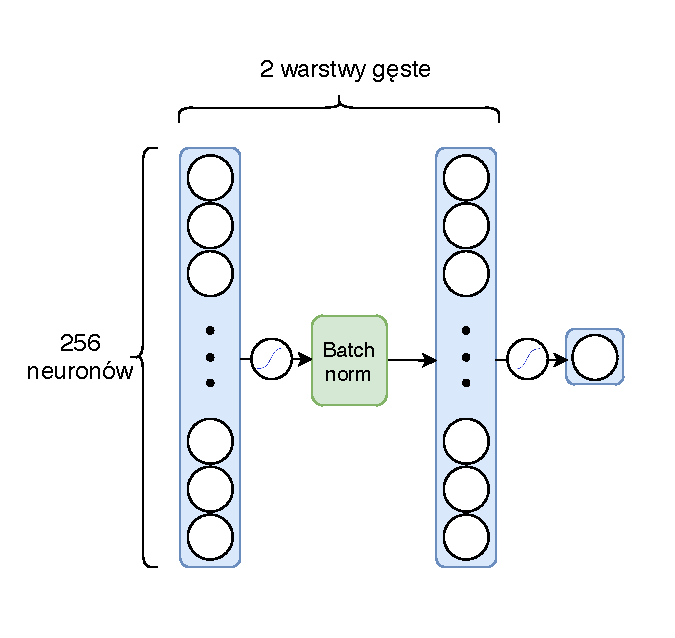
\includegraphics[width=0.7\textwidth]{best_neural_net.pdf}
	\caption{Zoptymalizowana sieć neuronowa (\textit{best-nn}). Składa się z dwóch ukrytych warstw gęstych oraz warstwy \textit{batch normalization}. Jako funkcji aktywacji użyto sigmoida.}
	\label{fig:nn2}
	\end{figure}	
	
	\section{XGBoost}
	Model oparty na XGBoost składał się ze 100 drzew decyzyjnych o maksymalnej głębokości 3. Wykorzystano stałą uczenia $\gamma = 10^{-1}$, funkcją kosztu była binarna entropia krzyżowa (tak samo jak w przypadku sieci neuronowych). Schematyczny rysunek architektury znajduje się na rysunku \ref{fig:xgb}.
	\begin{figure}
	\centering
	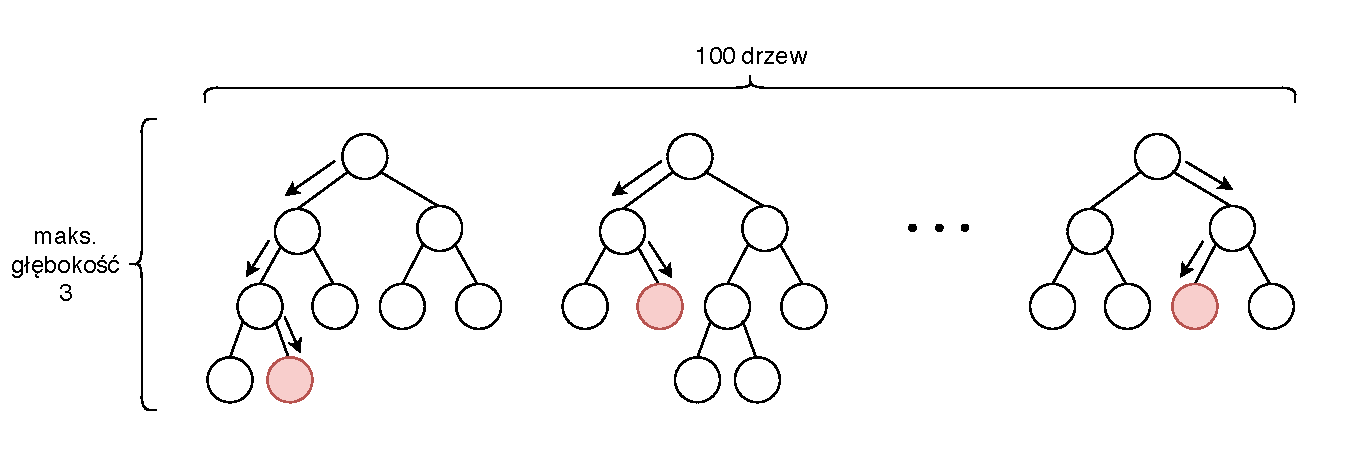
\includegraphics[width=1.0\textwidth]{xgb.pdf}
	\caption{Architektura modelu typu XGBoost opartego na drzewach decyzyjnych. Tutaj użyto modelu zawierającego 100 drzew o maksymalnej głębokości 3 (nie licząc korzenia).}
	\label{fig:xgb}
	\end{figure}
    
    \chapter{Wyniki}
    Każdy model trenowany był w dwóch trybach. Pierwszy z nich korzystał ze wszystkich zmiennych objaśniających, drugi zaś pomijał odpowiedzi klasyfikatorów. Dzięki temu można porównać wyniki z wcześniej używanymi modelami. Po dokonaniu analizy istotności zmiennych zauważono, że zmienna byCombinedIsolationDeltaBetaCorrRaw3Hits (patrz rozdział \ref{ch:dane}) jest najbardziej istotna dla wszystkich modeli. Jako, że rozkład tej zmiennej różni się na danych symulacyjnych oraz eksperymentalnych, postanowiono wytrenować również modele bez tej zmiennej.
    
	W tabeli \ref{tab:wyniki} znajdują się wyniki ROC AUC dla wszystkich modeli. Dla porównania zamieszczono wynik najlepszego z wcześniejszych klasyfikatorów, którym okazał się deepTau2017v1tauVSjet (później nazywany \textit{deepTau}). 
	
	Można zauważyć, że model oparty o XGBoost osiąga najwyższą skuteczność spośród zaproponowanych oraz wcześniej używanych modeli. W szczególności przy treningu na danych z wyłączeniem klasyfikatorów zarówno \textit{best-nn} jak i \textit{XGBoost} osiągnęły lepsze wyniki niż \textit{deepTau}. Widać również, że wyrzucenie głównej zmiennej nie pogarsza znacząco skuteczności modeli, a może skutkować lepszymi wynikami na danych eksperymentalnych. Ponadto, model oparty o same klasyfikatory osiąga lepszy wynik niż każdy klasyfikator osobno.
	
	
	\begin{table}[H]
	\centering
	\caption{Wartość ROC AUC dla wszystkich modeli na zbiorze testowym, pogrubioną czcionką zaznaczono najlepszy wynik.}
	\label{tab:wyniki}
	\begin{tabular}{lrrrrr}
	\toprule
	Tryb & \textit{baseline} & \textit{best-nn} & \textit{XGBoost} & \textit{deepTau} & \textit{ensemble} \\
	\midrule
	Pełne dane & .9948 & .9979 & \textbf{.9985} & $-$ & $-$ \\
	Bez klas. & .9940 & .9949 & \textbf{.9956} & .9945 & $-$  \\
	Bez najlepszej & .9977 & .9972 & \textbf{.9985} & $-$ & $-$ \\
	Same klas. & $-$ & $-$ & $-$ & $-$ & .9956 \\
	\bottomrule
	\end{tabular}
	\end{table}

	
	Na rysunkach \ref{fig:res_best}, \ref{fig:res_new} i \ref{fig:res_disc} przedstawiono fragmenty krzywych ROC dla wybranych modeli. Na wykresach osie są zamienione, więc lepszy model ma mniejsze pole pod krzywą. Zakres TPR na wykresach został zmniejszony, aby lepiej uwidocznić różnice między modelami.
	
	
	\begin{figure}[H]
	\centering
	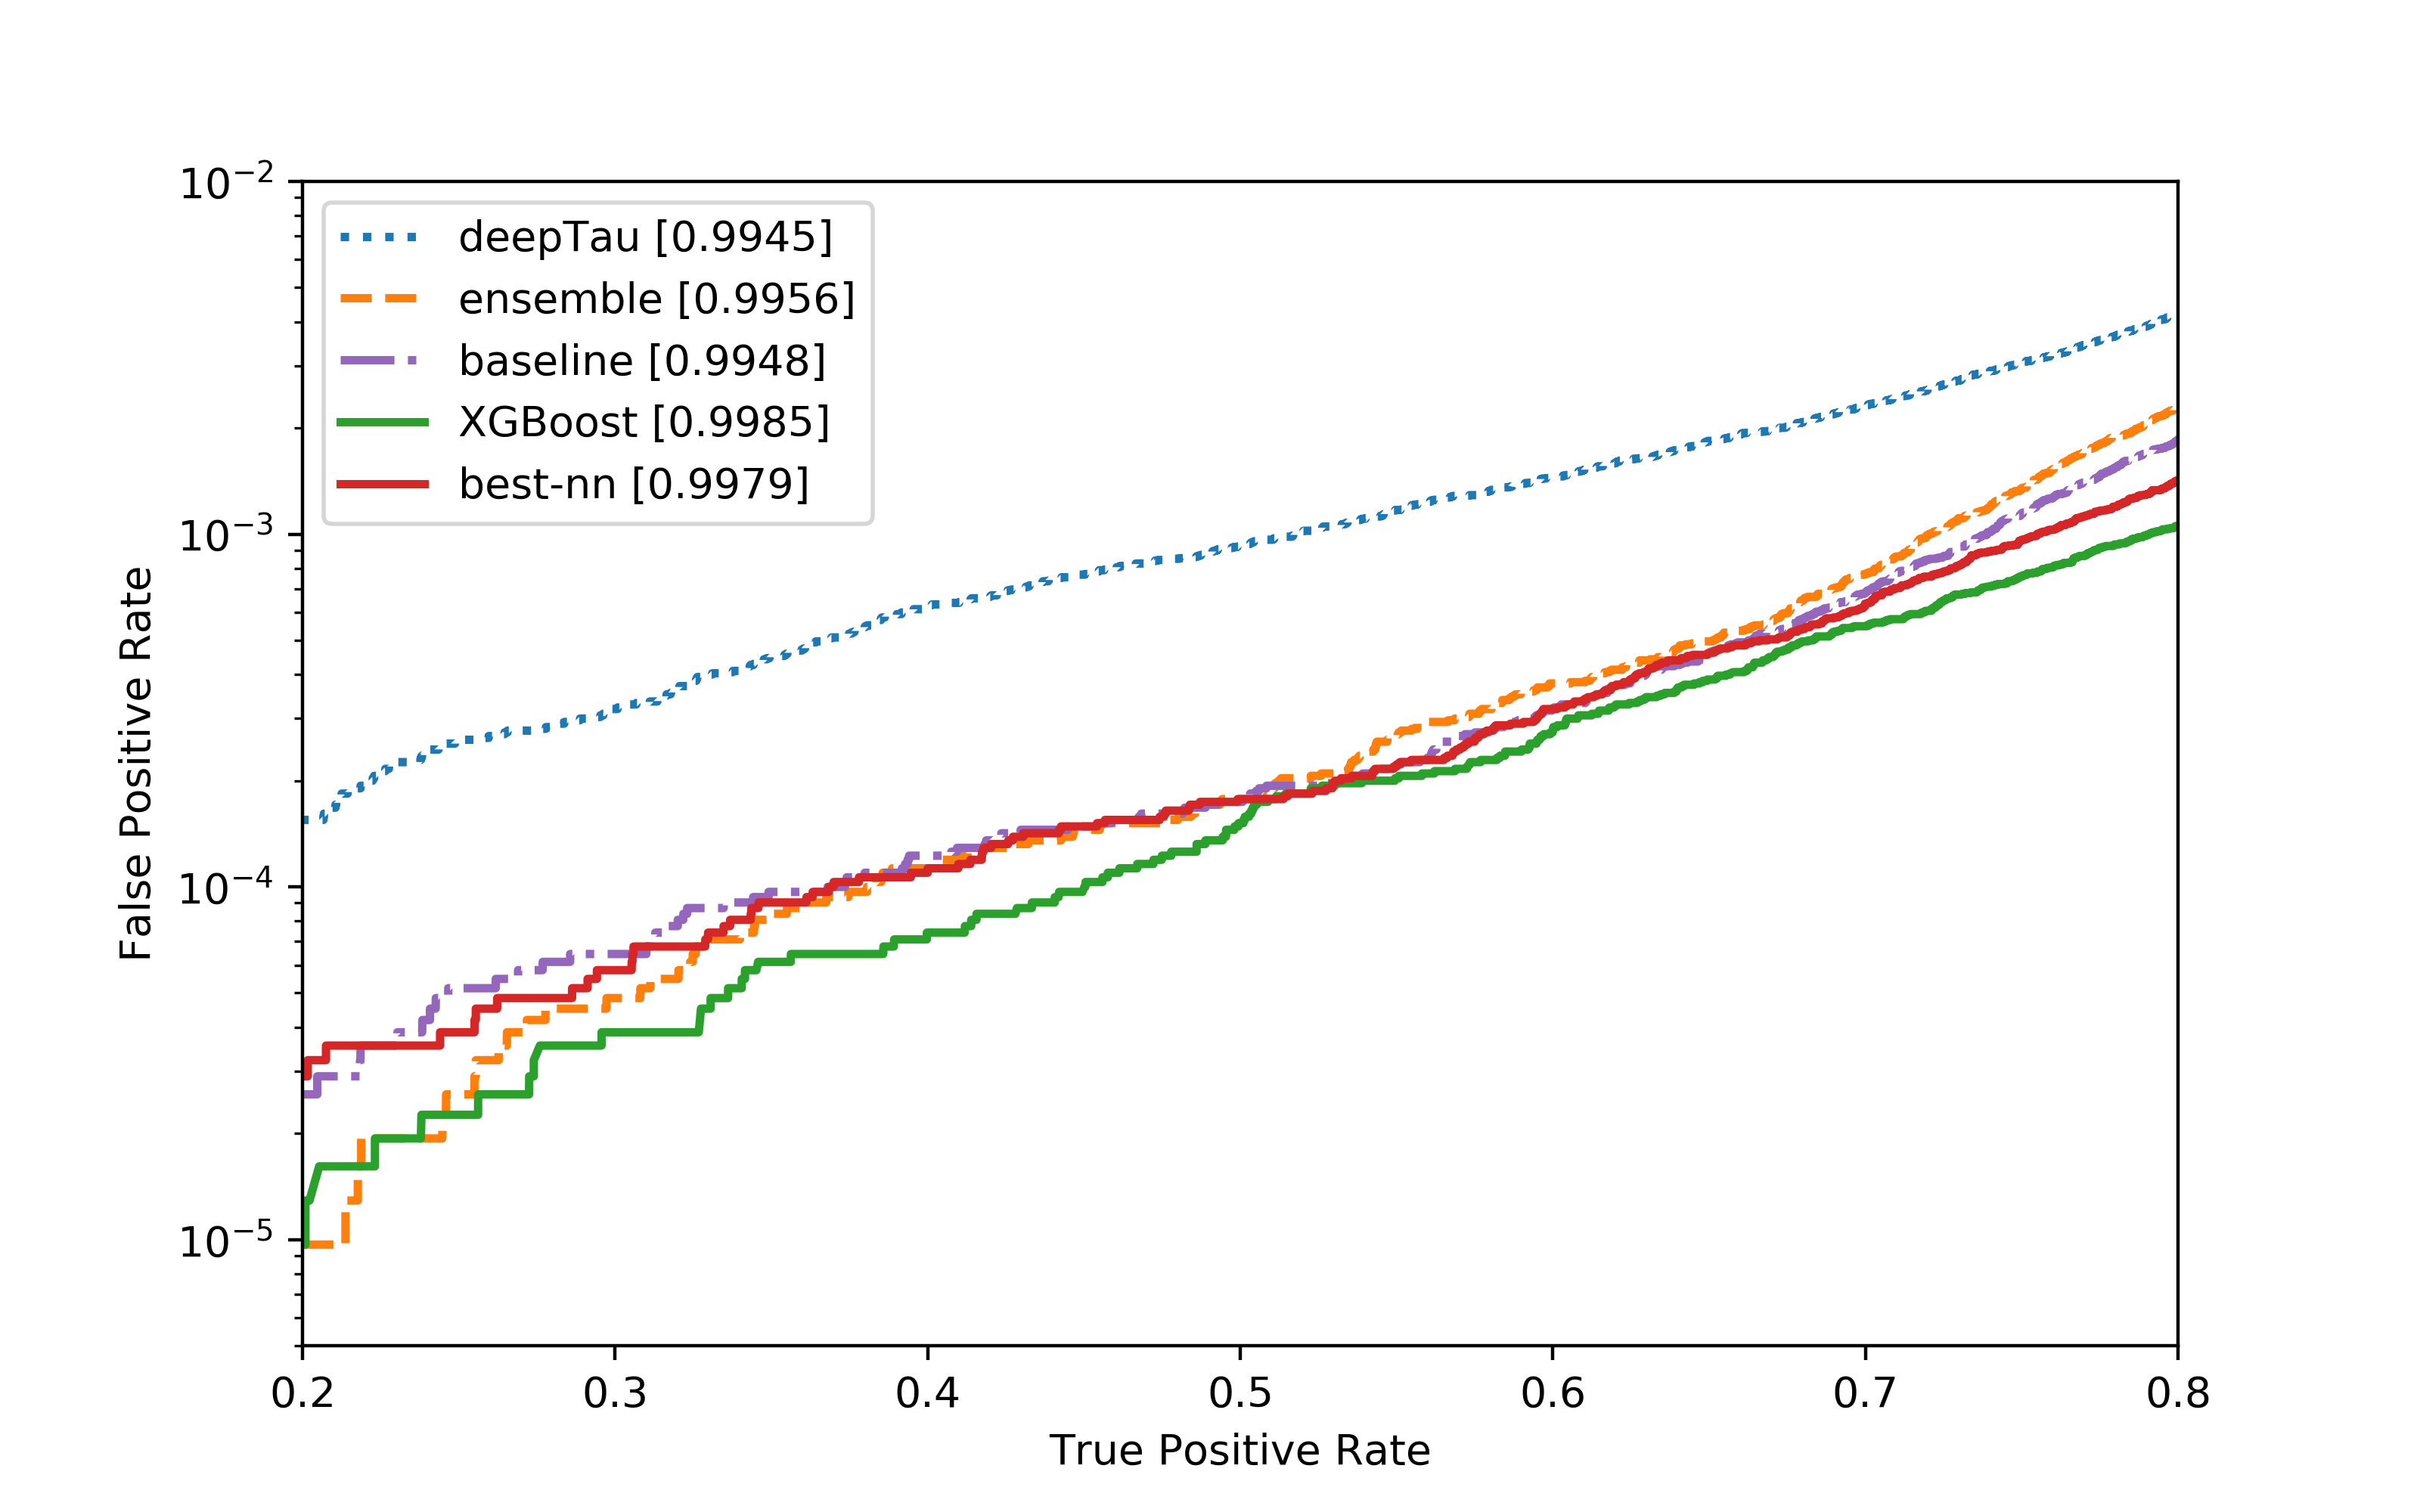
\includegraphics[width=1\textwidth]{best_models.png}
	\caption{Porównanie najlepszych modeli na podstawie krzywej ROC.  \textit{baseline}, \textit{best-nn} oraz \textit{XGBoost} były uczone na pełnych danych, a \textit{deepTau} na danych bez klasyfikatorów. W nawiasach kwadratowych podano wartość ROC AUC dla danego modelu.}
	\label{fig:res_best}	
	\end{figure}
	
	Na rysunku \ref{fig:res_best} przedstawiono najlepsze modele każdego typu. Można zauważyć, że największa różnica jest między \textit{deepTau} a innymi modelami, natomiast najskuteczniejszy jest \textit{XGBoost}. Na tym fragmencie krzywej różnice między wytrenowanymi modelami są dosyć niewielkie.
	
	\begin{figure}[H]
	\centering
	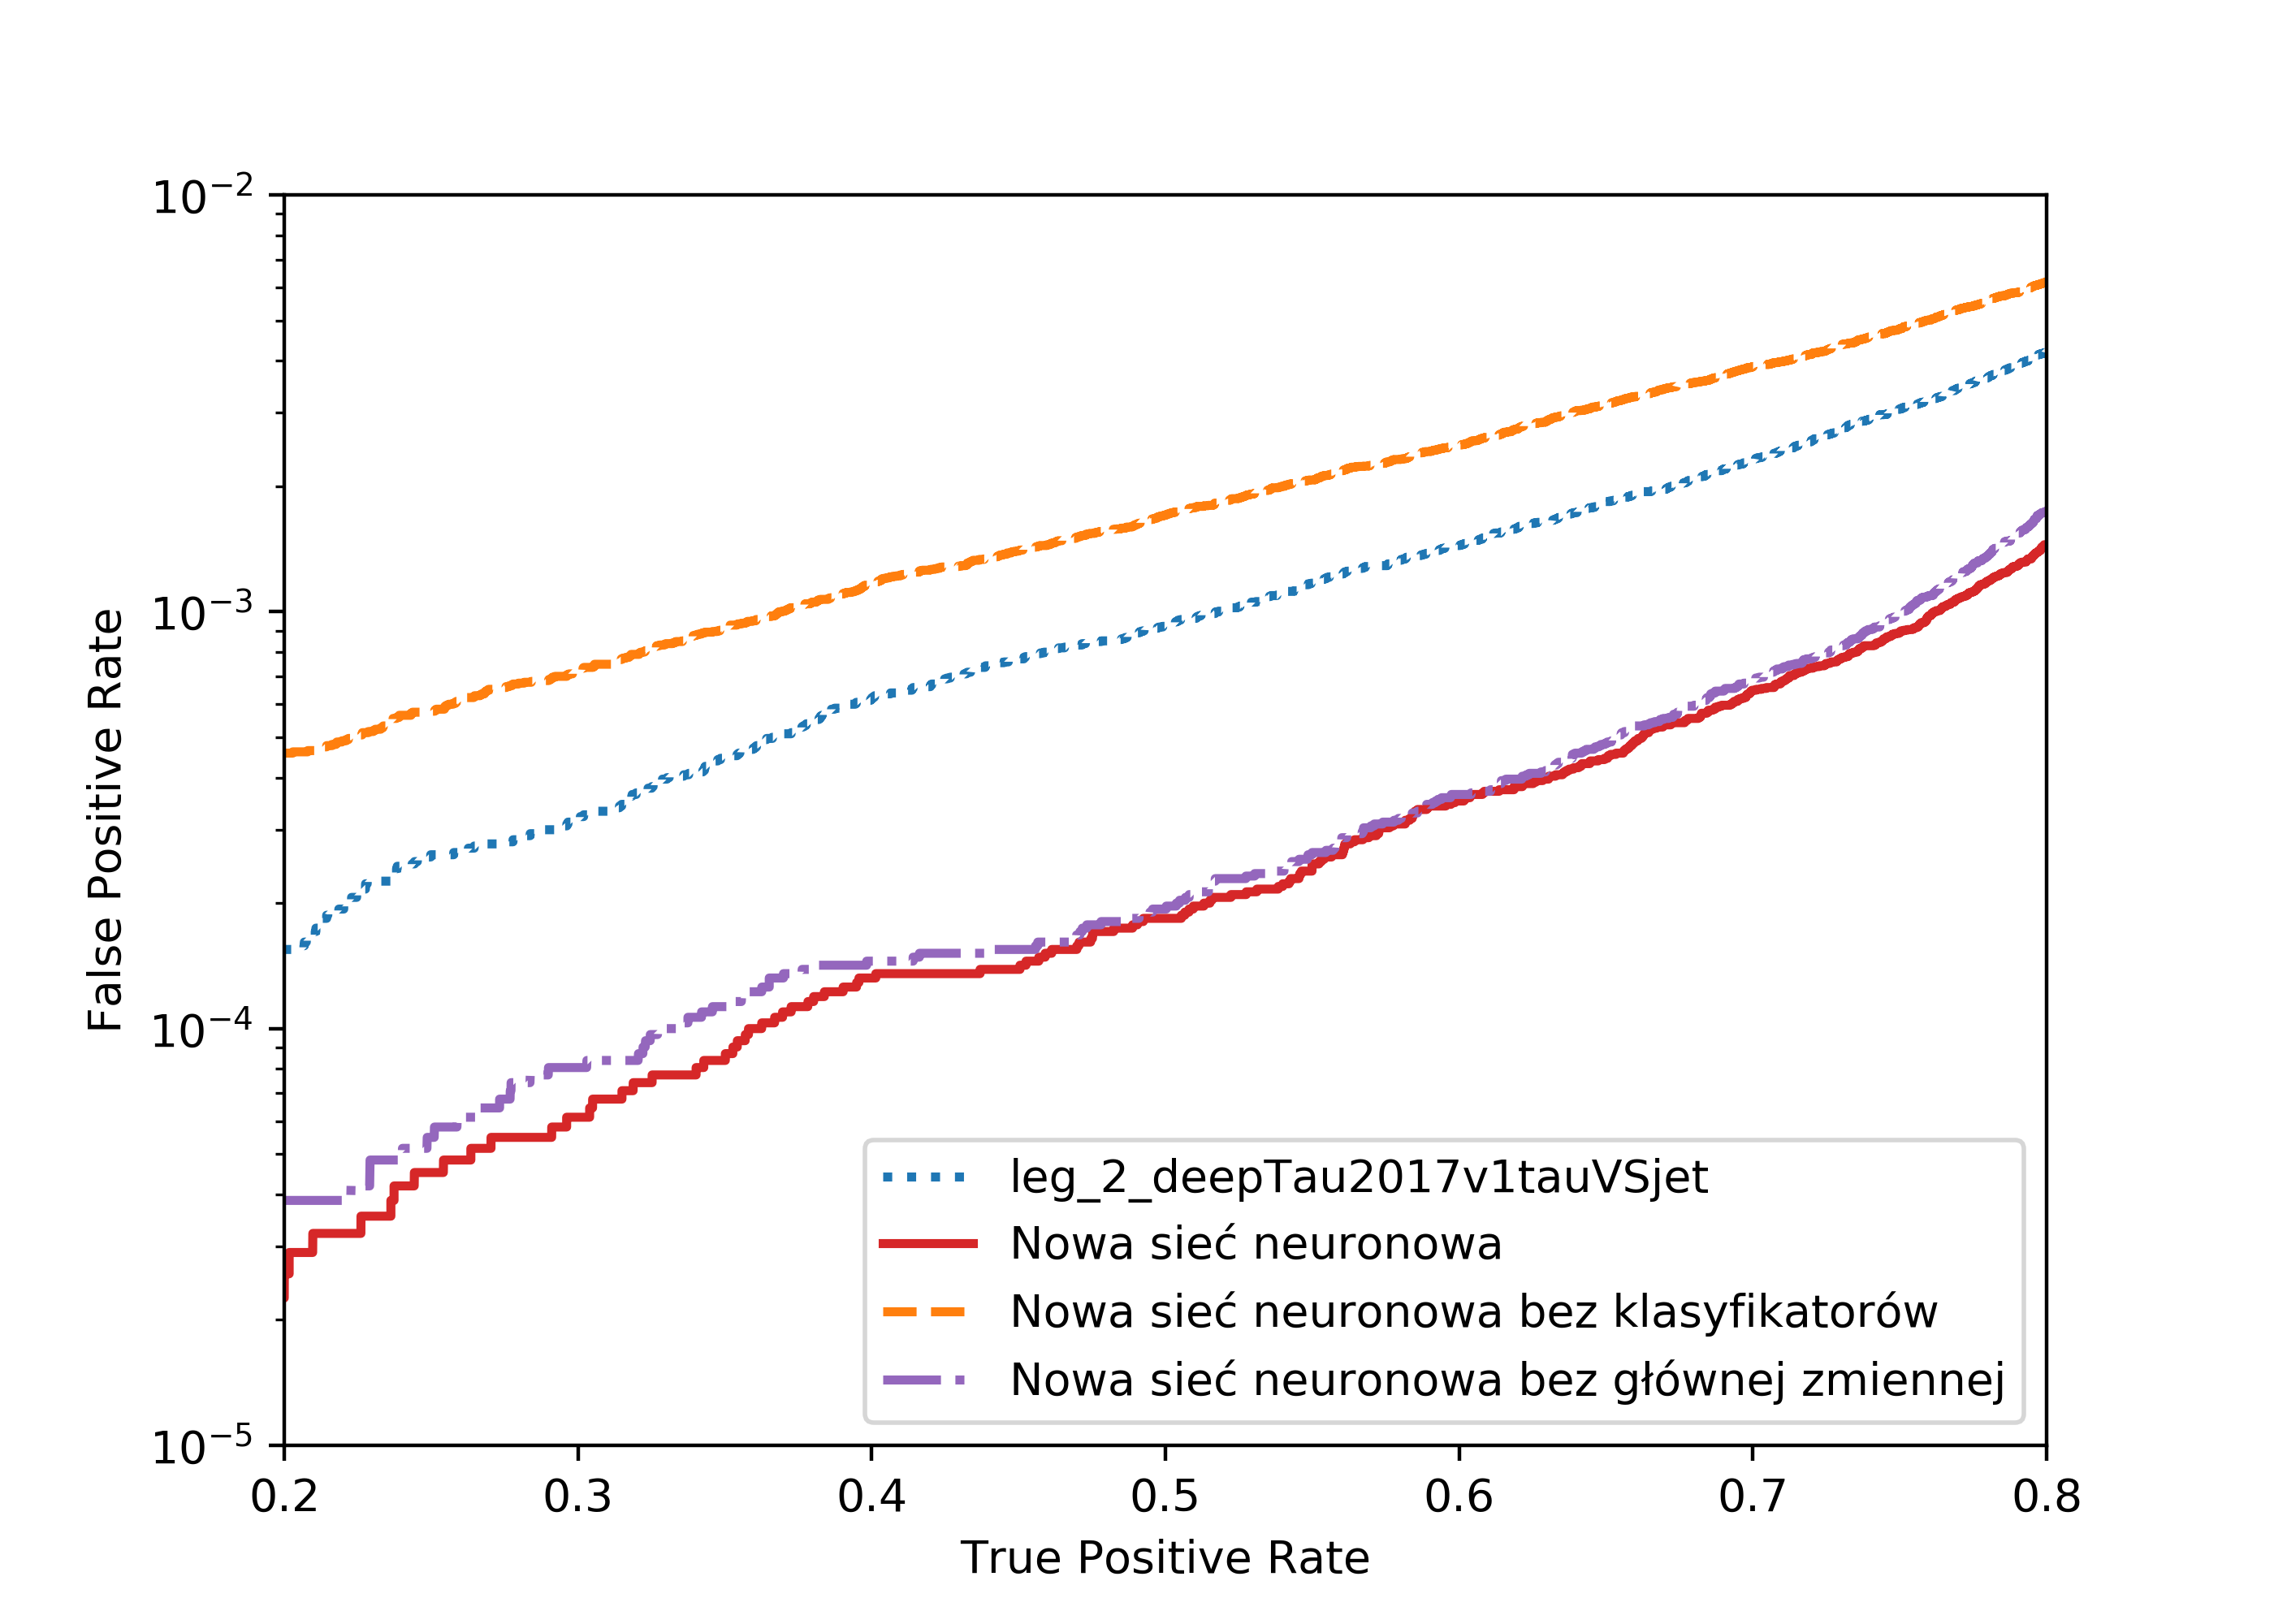
\includegraphics[width=1\textwidth]{new_network.png}
	\caption{Porównanie wszystkich trybów uczenia nowej sieci z najlepszym klasyfikatorem na podstawie krzywej ROC. W nawiasach kwadratowych podano wartość ROC AUC dla danego modelu.}
	\label{fig:res_new}	
	\end{figure}
	
	Na rysunku \ref{fig:res_new} znajdują się wszystkie tryby treningu nowej sieci w porównaniu z \textit{deepTau}. Wyniki dla treningu na pełnych danych i z wyłączeniem głównej zmiennej nie różnią się znacząco, natomiast trening bez klasyfikatorów widocznie pogarsza wygląd krzywej ROC. Na tym fragmencie osiąga gorsze wyniki niż \textit{deepTau}. Jednak patrząc na wartość ROC AUC można podejrzewać, że osiąga lepsze rezultaty na skrajnych fragmentach.
	
	\begin{figure}[H]
	\centering
	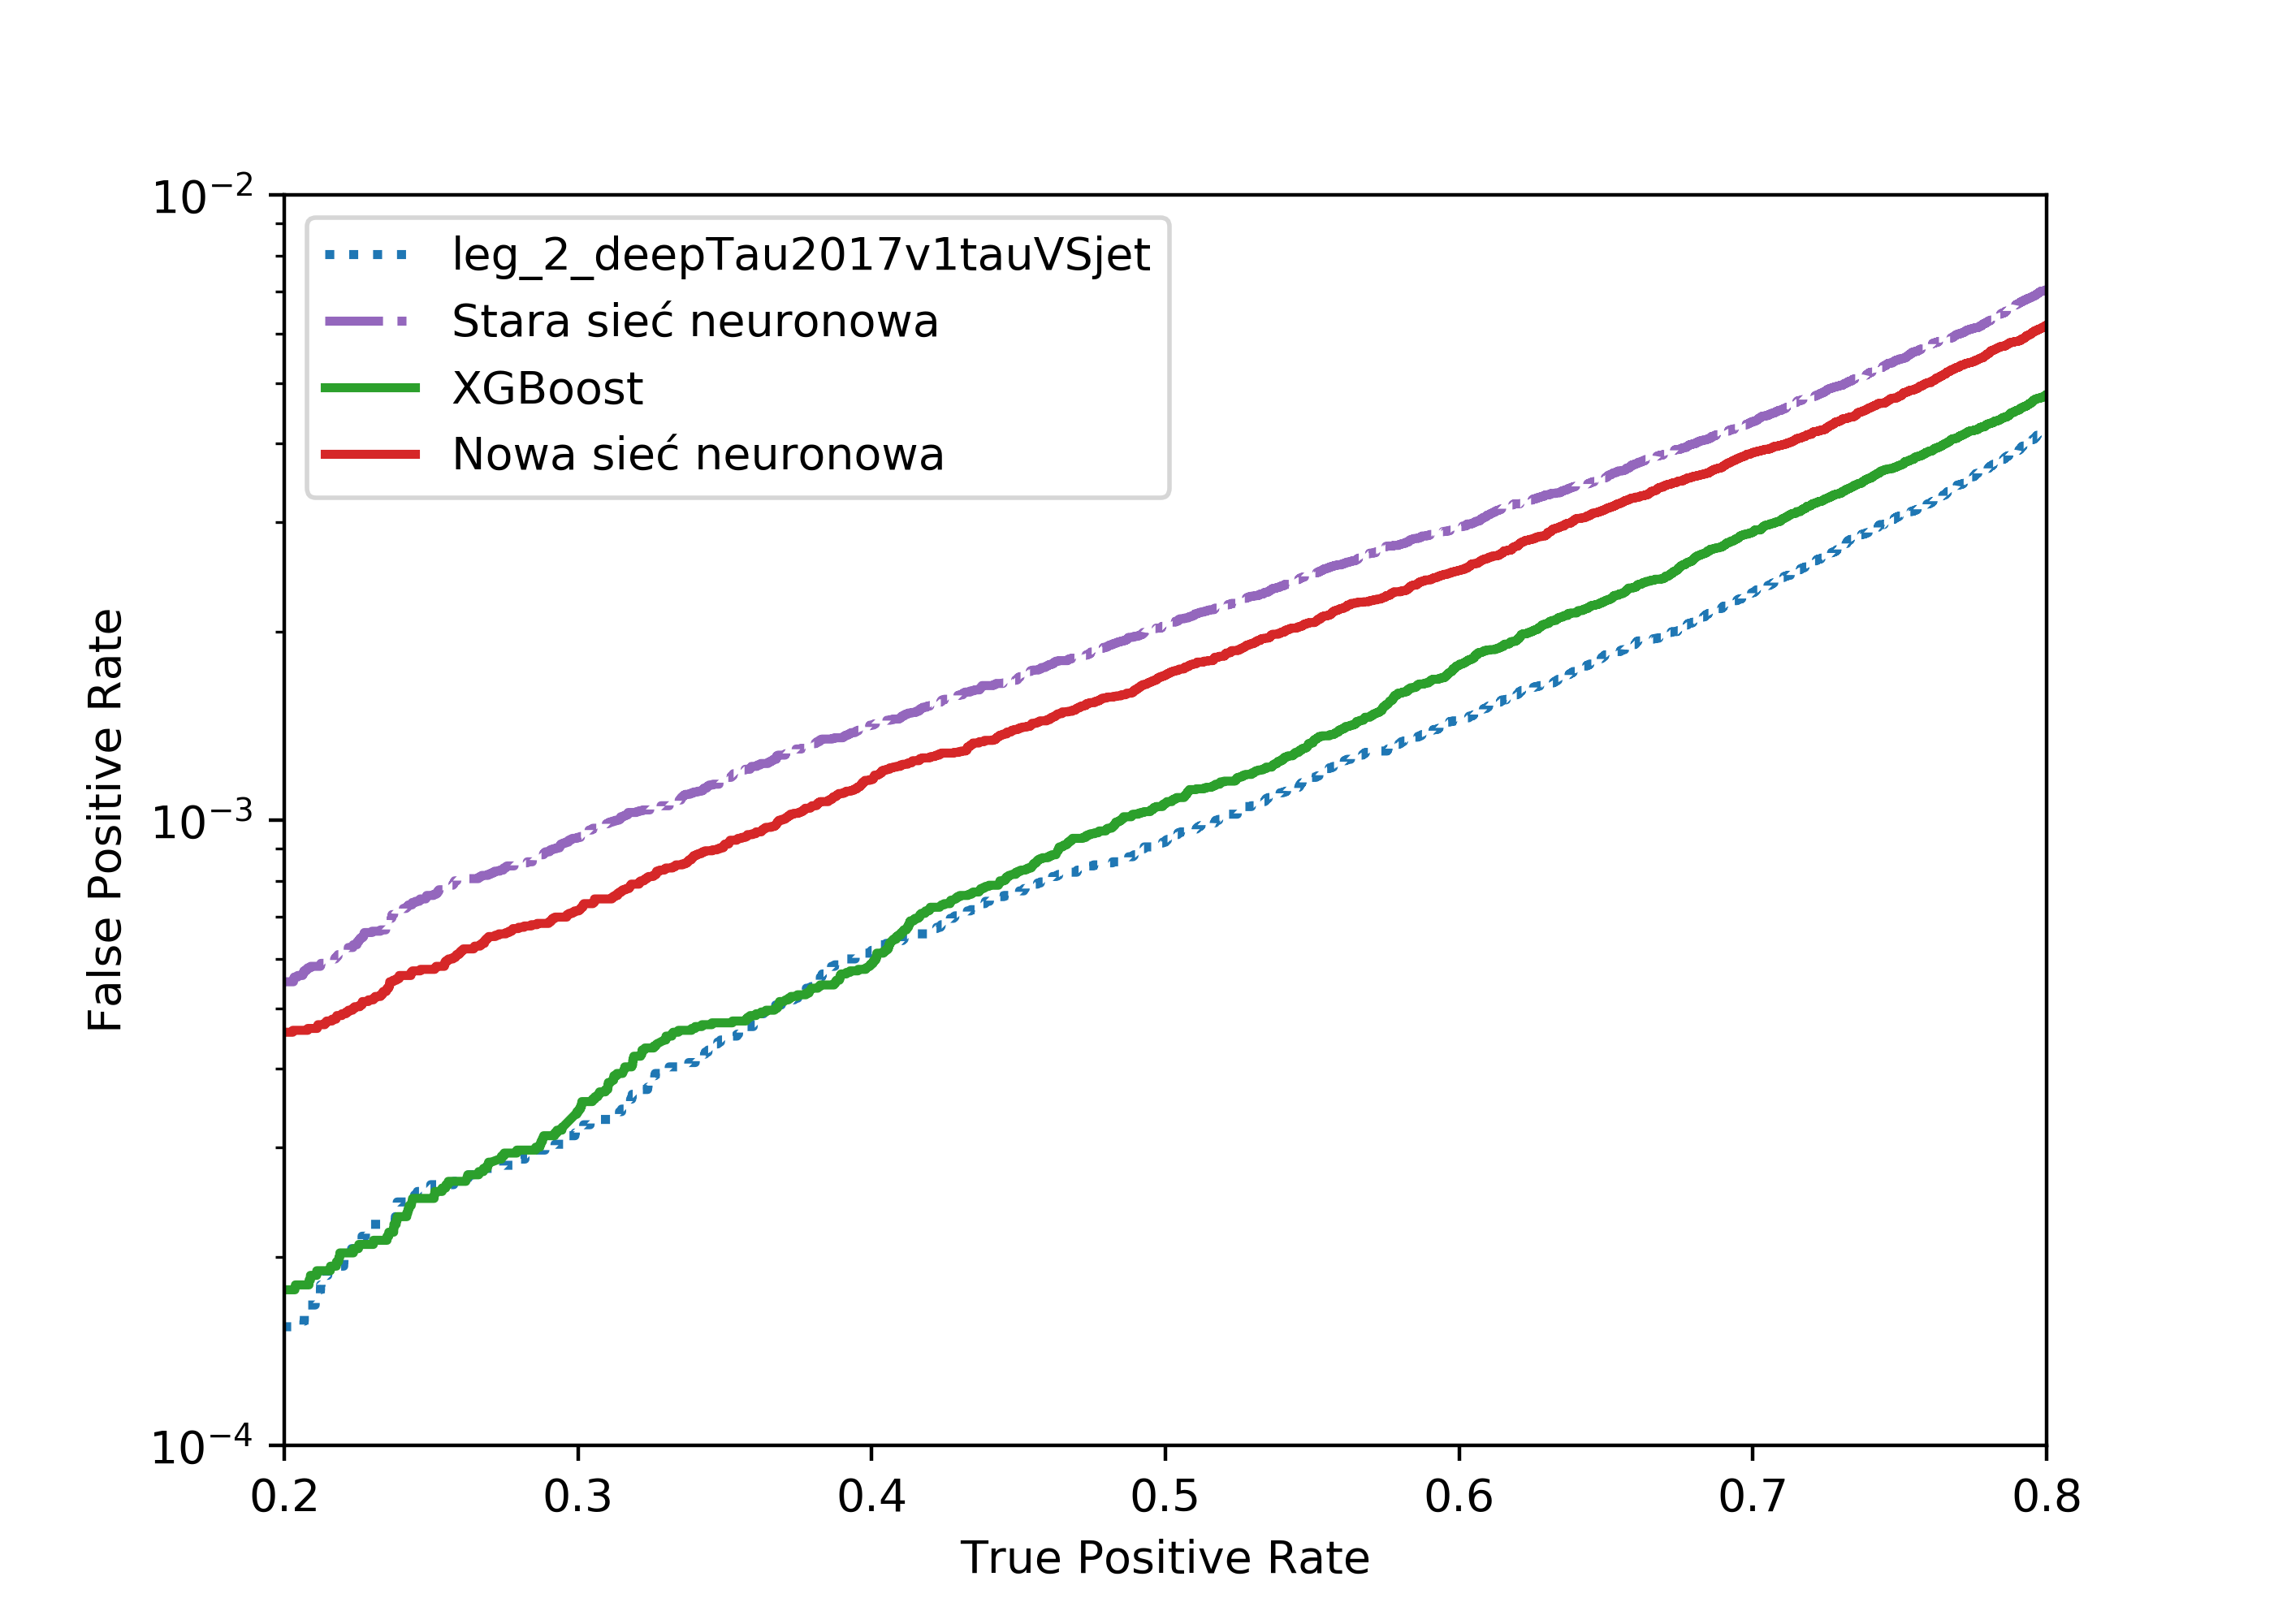
\includegraphics[width=1\textwidth]{without_disc.png}
	\caption{Porównanie modeli uczonych na danych bez klasyfikatorów na podstawie krzywej ROC. W nawiasach kwadratowych podano wartość ROC AUC dla danego modelu.}
	\label{fig:res_disc}
	\end{figure}
	
	Na rysunku \ref{fig:res_disc} widnieje porównanie każdego typu modelu uczonego na danych bez klasyfikatorów. Można zauważyć, że na wyróżnionym fragmencie najlepsze wyniki osiąga \textit{deepTau}, jednak są one zbliżone do wyników \textit{XGBoosta}. Patrząc na wartości ROC AUC możemy przypuszczać, że zarówno \textit{XGBoost} jak i \textit{best-nn} uzyskują lepsze rezultaty niż \textit{deepTau} na skrajnych zakresach TPR.
	
	%TODO wielkość wykresów
    
    \chapter{Dyskusja}
    
	Porównując dane symulacyjne i eksperymentalne można zauważyć również różnice w rozkładach zmiennych objaśniających, także nie ma pewności, że model dający dobre wyniki na danych symulacyjnych będzie dawał równie dobre wyniki na danych eksperymentalnych.	Jest to jednak jedyne dostępne źródło danych.	
	
    \chapter{Podsumowanie}
    
    \addcontentsline{toc}{chapter}{Bibliografia}
    \printbibliography
    
\end{document}
